% Section content template for individual Educative lessons
% This file contains the actual content for a specific section
% Generated from Educative API section content

% Section: Requirements for Facebook
% Section ID: 5451109412110336
% Section Slug: requirements-for-facebook
% Generated: 2025-12-14T12:38:42.194373

In this lesson, we'll list the requirements of Facebook. This is a very crucial step, as requirements define the scope of a problem, so getting them right from the interviewer and understanding them well will make the design of the rest of the system smooth and easy.
\\
We'll use the notational convention to identify each requirement with a unique label ``Rn,'' where ``R'' is short for requirement and ``n'' is a natural number.

\subsection{Requirements collection}\label{rl0q9rFTxzahkmjgF9tuX}
\\
The requirements for Facebook are defined below:

% \vspace{-1.0\baselineskip}
\noindent
\begin{minipage}[t]{0.48\textwidth}\vspace{0pt}
\textbf{R1:} Users should be able to create and edit their profile page by adding personal details such as name, address, phone number, and email. They should also be able to add multiple entries for work experience, education, and places of living. Users should also be able to set the privacy of their profile page.
\\
\textbf{R2:} Our system's users should be able to search for groups, pages, and other users.
\end{minipage}
\hfill
\begin{minipage}[t]{0.48\textwidth}\vspace{0pt}
\centering
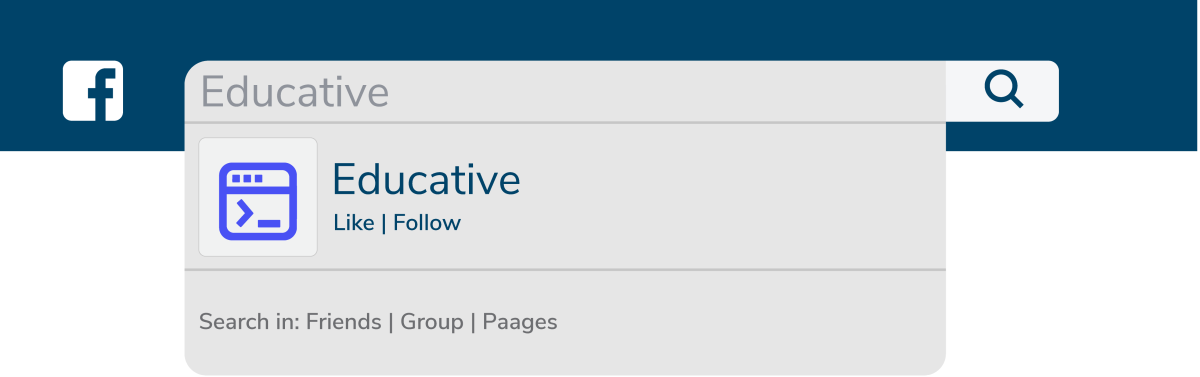
\includegraphics[width=0.5\textwidth]{Images/chapter_22/section_5451109412110336/5039926821519360.png}
\end{minipage}

% \vspace{-1.0\baselineskip}
\noindent
\begin{minipage}[t]{0.48\textwidth}\vspace{0pt}
\textbf{R3:} Users should be able to write a new post and set its privacy.
\\
\textbf{R4:} Users should be able to send and respond to other users' friend requests. Users should also be able to unfriend or block other users.
\\
\textbf{R5:} Users should be able to follow other users without adding them to their friend list.
\end{minipage}
\hfill
\begin{minipage}[t]{0.48\textwidth}\vspace{0pt}
\centering
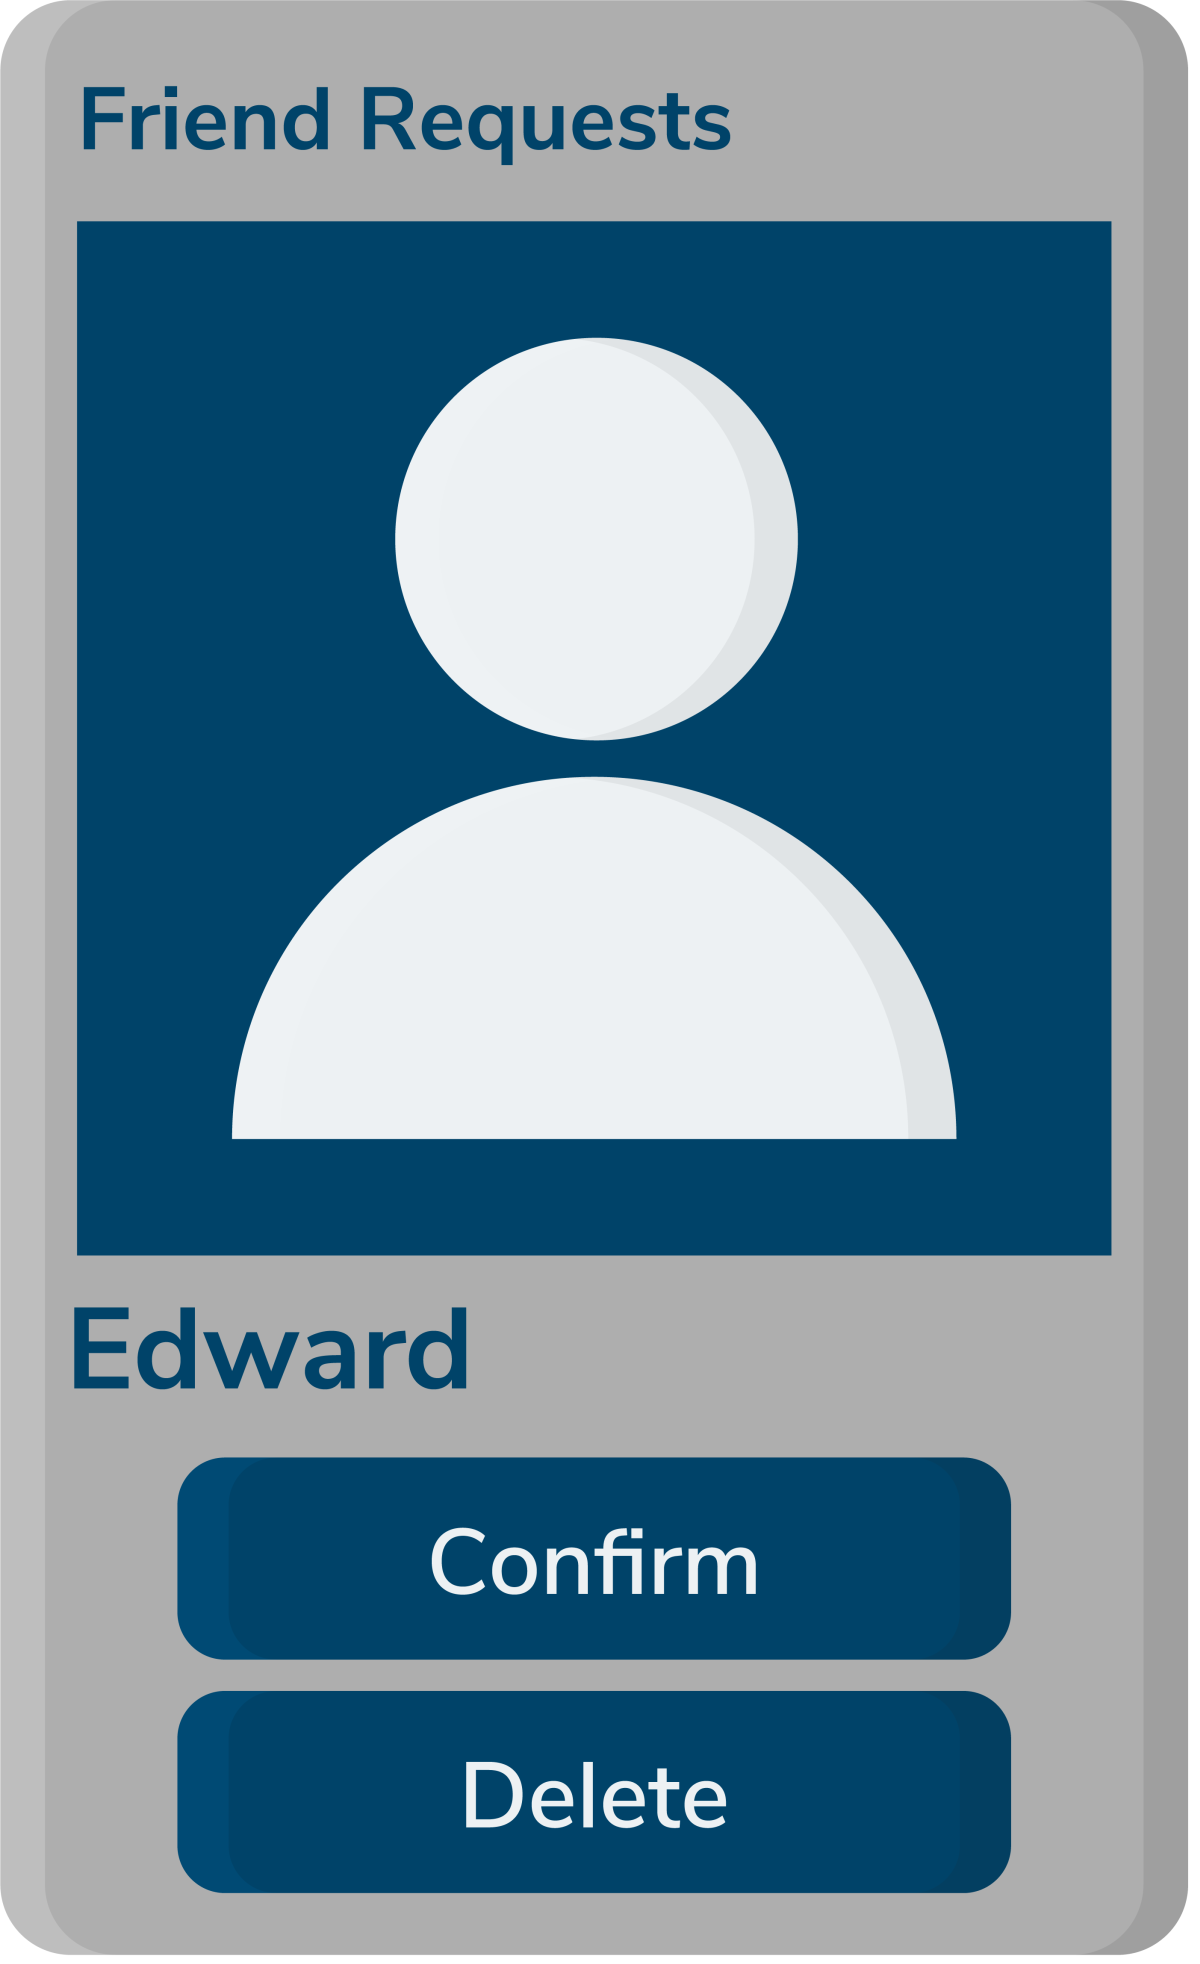
\includegraphics[width=0.5\textwidth]{Images/chapter_22/section_5451109412110336/6228896078102528.png}
\end{minipage}

% \vspace{-1.0\baselineskip}
\noindent
\begin{minipage}[t]{0.48\textwidth}\vspace{0pt}
\textbf{R6:} Users should be able to like, share, and comment on posts and existing comments.
\\
\textbf{R7:} The system should notify the user whenever there has been an interaction with them, such as receiving a message, a friend request, or a comment on their post.
\end{minipage}
\hfill
\begin{minipage}[t]{0.48\textwidth}\vspace{0pt}
\centering
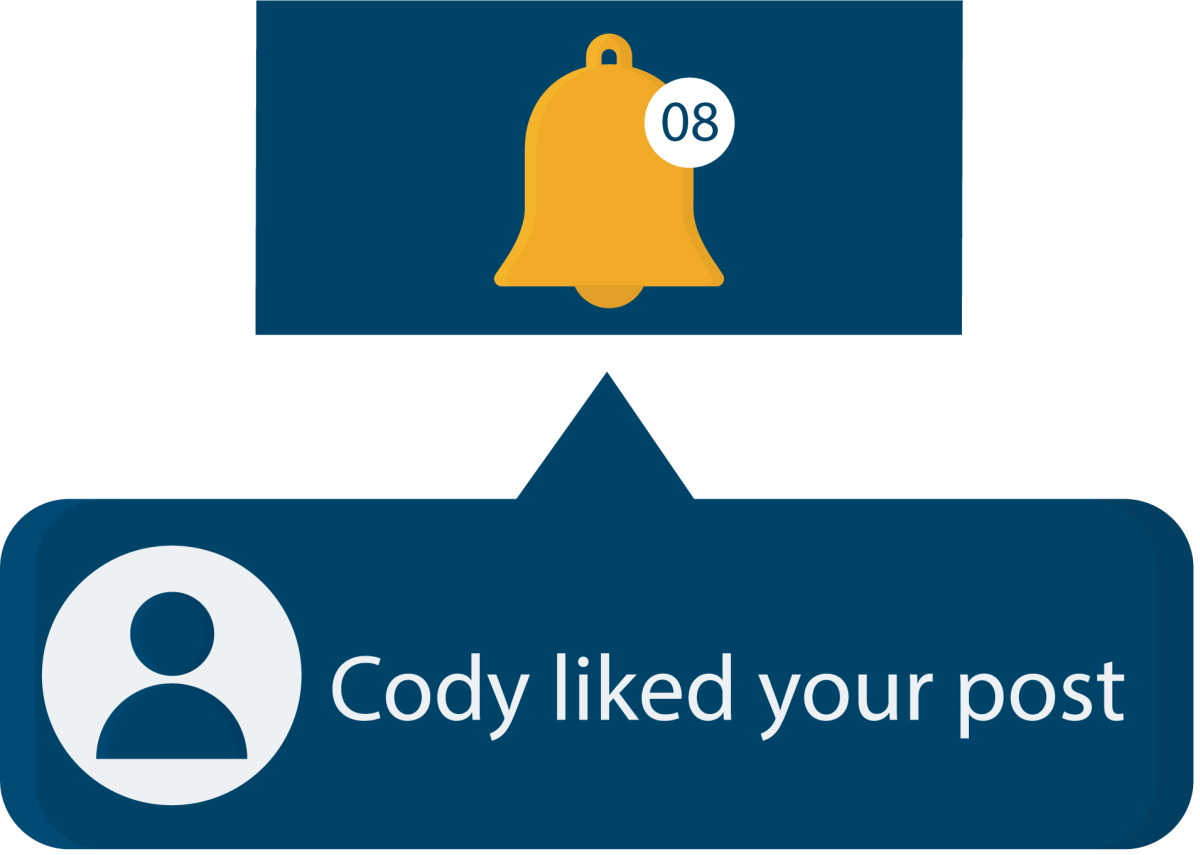
\includegraphics[width=0.5\textwidth]{Images/chapter_22/section_5451109412110336/4809152494043136.png}
\end{minipage}

% \vspace{-1.0\baselineskip}
\noindent
\begin{minipage}[t]{0.48\textwidth}\vspace{0pt}
\textbf{R8:} A user should be able to send and receive messages from other users.
\\
\textbf{R9:} Users should be able to follow existing pages and join existing groups. They should also be able to unfollow or leave joined groups or followed pages.
\\
\textbf{R10:} Users should be able to create their groups and pages. Users can later set privacy or delete the groups or pages they own.
\end{minipage}
\hfill
\begin{minipage}[t]{0.48\textwidth}\vspace{0pt}
\centering
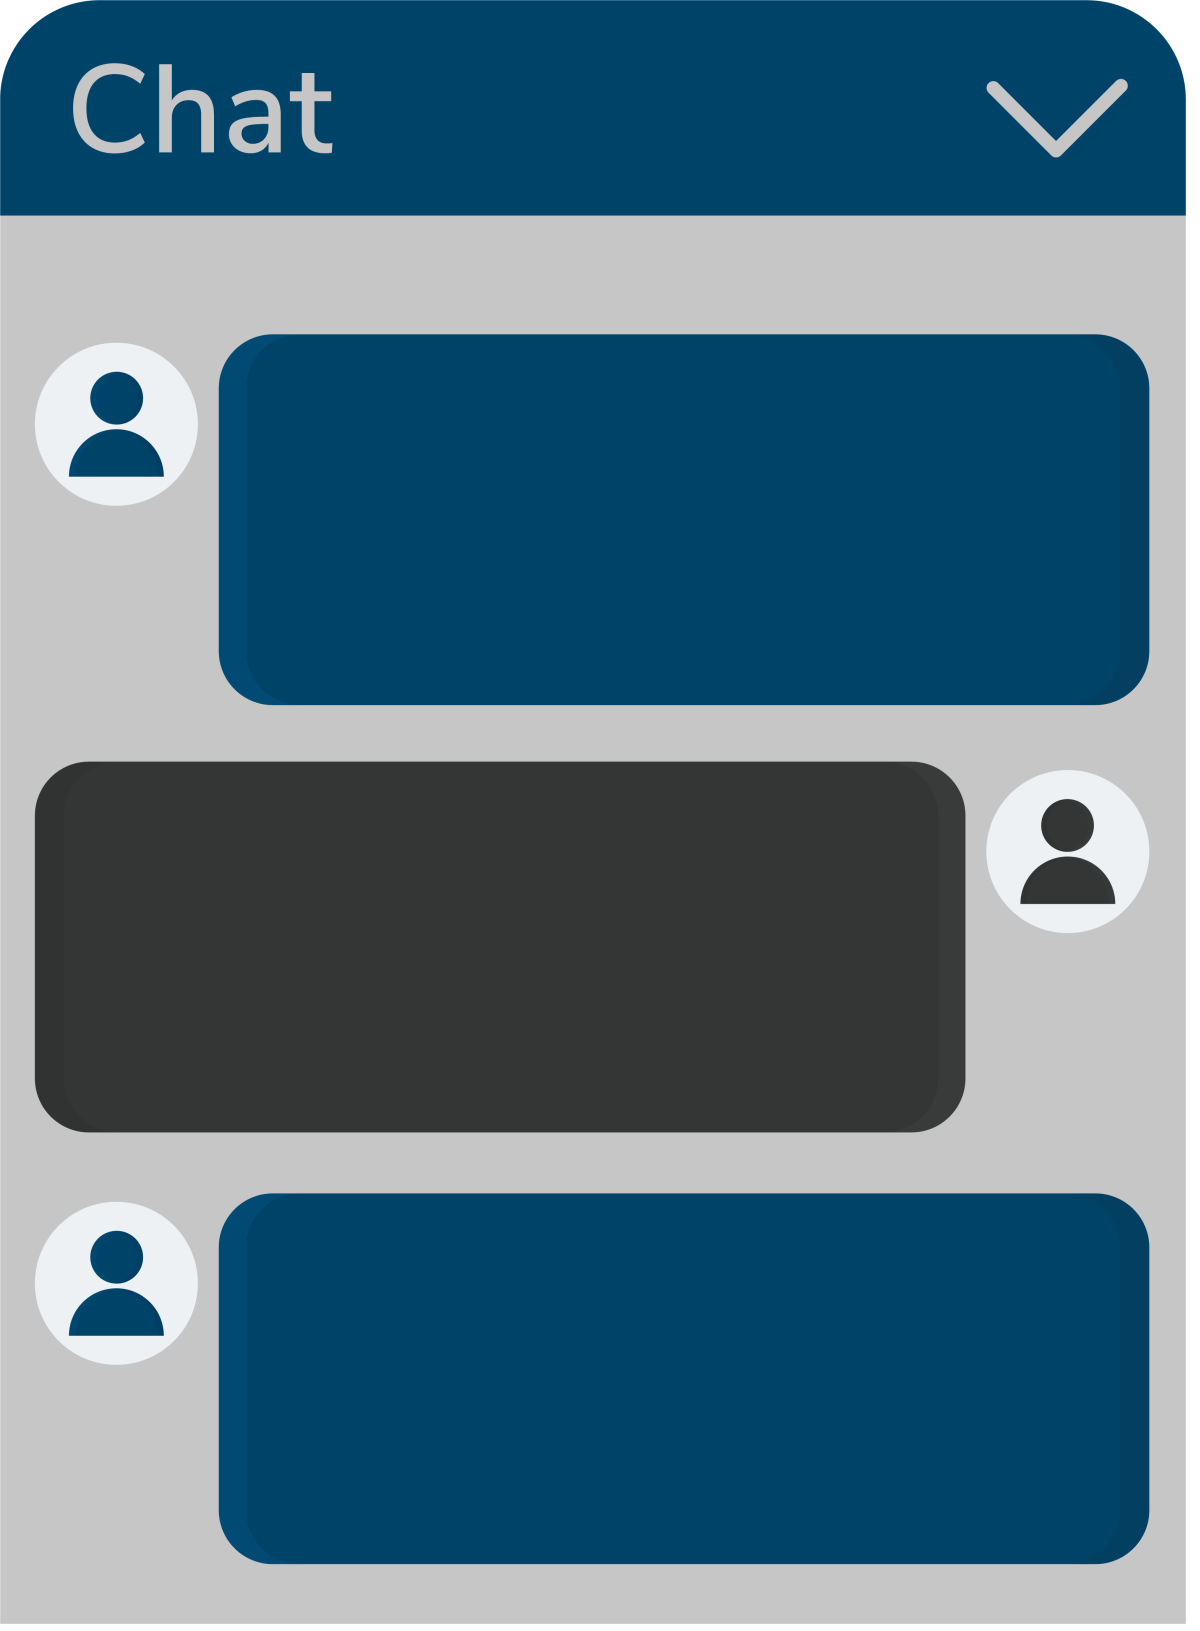
\includegraphics[width=0.5\textwidth]{Images/chapter_22/section_5451109412110336/6056620242239488.png}
\end{minipage}

We've identified our requirements for the problem, and in the next lesson, we will define different use cases of Facebook.

% End of section content